\chapter{Detekcja obiektów}
\label{ch:detekcja}
W poprzednim rozdziale przedstawiono wymagania konkursu DAC SDC 2021 oraz jego główne zadanie -- detekcję obiektów. 
W niniejszym rozdziale przedstawione zostaną metody detekcji -- klasyczne oraz bazujące na sieciach neuronowych, 
a także architektury sieci stosowane w~rozwiązaniach energooszczędnych, w~tym sieci kwantyzowane (ang. \emph{Quantized Neural Networks}, \emph{QNN}) oraz binarne (ang. \emph{Binary Neural Networks}, \emph{BNN}).

\section{Zadanie detekcji}

Analizę rozważanego zadania należy rozpocząć od jego sformułowania. 
Zakładając, iż dany jest obraz $F(y,x)$ 
o szerokości $W$ i~wysokości $H$
określony na zbiorze 
\begin{equation}
D = \{(y,x) \in \mathbb{N} ^2 : 0 \leq x < W \land 0 \leq y < H\}
\end{equation}
stanowiącym zbiór pikseli obrazu (par współrzędnych) $(y,x)$ 
oraz $P \subseteq D$ oznaczające zbiór pikseli poszukiwanego obiektu, należy znaleźć $x_{min},x_{max},y_{min}$ oraz $y_{max}$ takie, że spełnione są zależności \eqref{eq:xmin}-\eqref{eq:ymax}.
Na rysunku \ref{fig:det_grid} przedstawiono graficzną interpretację poniższych równań.
\begin{equation}
x_{min} = \min_{j \in \mathbb{N} \land j < W }\{j : \exists i \in \mathbb{N} \land i < H \land (i,j) \in P \}
\label{eq:xmin}
\end{equation}
\begin{equation}
x_{max} = \max_{j \in \mathbb{N} \land j < W }\{j : \exists i \in \mathbb{N} \land i < H  \land (i,j) \in P \}
\label{eq:xmax}
\end{equation}
\begin{equation}
y_{min} = \min_{i \in \mathbb{N} \land i < H }\{i : \exists j \in \mathbb{N} \land j < W \land (i,j) \in P \}
\label{eq:ymin}
\end{equation}
\begin{equation}
y_{min} = \max_{i \in \mathbb{N} \land i < H }\{i: \exists j \in \mathbb{N} \land j < W \land (i,j) \in P \}
\label{eq:ymax}
\end{equation}

Innymi słowy należy znaleźć parametry:
\begin{equation}
bbox = (x_{min},x_{max},y_{min},y_{max})
\label{eq:bbox_xxyy}
\end{equation}
najmniejszego prostokąta opisanego (ang. \emph{bounding box}) na poszukiwanym obiekcie.
Możliwa jest również inna reprezentacja
\begin{equation}
bbox = (x_c,y_c, w,h)
\label{eq:bbox_xywh}
\end{equation}
gdzie kolejne zmienne to współrzędne  środka  oraz wymiary obiektu. Obie reprezentacje wiązane są poprzez równania \eqref{eq:xc}-\eqref{eq:height}.
\begin{equation}
x_c = \frac{x_{min} + x_{max}}{2}
\label{eq:xc}
\end{equation}
\begin{equation}
y_c = \frac{y_{min} + y_{max}}{2}
\label{eq:yc}
\end{equation}
\begin{equation}
w = x_{max} - x_{min}
\label{eq:width}
\end{equation}
\begin{equation}
h = y_{max} - y_{min}
\label{eq:height}
\end{equation}

\begin{figure}
    \centering
    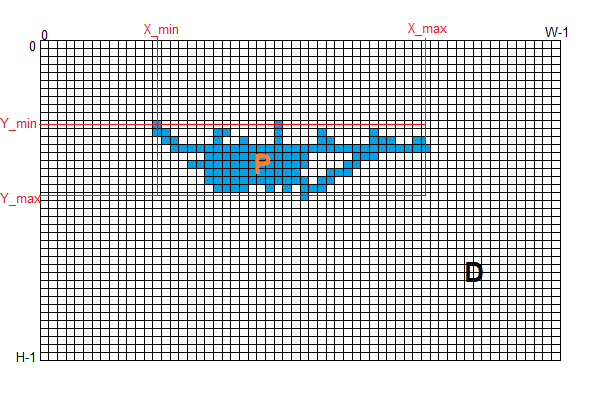
\includegraphics[width=0.9\linewidth]{images/grid_obj.png}
    \caption{Graficzna interpretacja zadania detekcji.}
    \label{fig:det_grid}
\end{figure}

Przedstawione sformułowanie zadania tyczy się detekcji pojedynczego obiektu z~założeniem, iż obiekt znajduje się na obrazie. 
W przypadku ogólnym należy znaleźć $n$ \emph{bounding box}, przy czym $n$ jest zmienne i~zależne od rozpatrywanego obrazu.
Bardzo często zadanie detekcji łączone z~zadaniem klasyfikacji, wówczas oprócz położenia i~wymiarów obiektu należy podać również jego typ/klasę. 

\section{Metody klasyczne}

W prostych przypadkach zadanie detekcji może sprowadzić się do znalezienia wymiarów obiektów na obrazie binarnym.
% , uzyskanym np. w~wyniku segmentacji. 
Sytuacja tak może mieć miejsce, gdy poszukiwany obiekt znacząco odróżnia się od tła.
Wówczas możliwe jest wskazanie pikseli należących do rozpatrywanego obiektu, poprzez np. binaryzację na podstawie wybranych składowych przestrzeni barwnej.
Możliwe są również rozwiązania wykorzystujące technikę okna przesuwnego, ekstrakcji wybranych cech wraz z~zadaniem klasyfikacji.
Wówczas mamy do czynienia z~tzw. metodami klasycznymi.
Znalezienie parametrów $bbox$ możliwe wówczas jest z~użyciem algorytmów wizji komputerowej lub uczenia maszynowego.

Wspomniana technika okna przesuwnego jest realizowana poprzez analizę (klasyfikację) fragmentów obrazu (zwanych oknem) o~określonych wymiarach $(d_w,d_h)$. 
Fragmenty te stanowią otoczenie wybranych punktów obrazu.
Wybierane punty stanowią węzły siatki oddalone od siebie o~określoną wartość kroku $(s_w,s_h)$. 
Można to utożsamiać z~``przesuwaniem'' okna w~płaszczyźnie obrazu.
W przedstawionej technice rozmiar okna jest stały co powoduje, że obiekty o~wymiarach innych, niż 
rozpatrywane w~problemie klasyfikacji mogą nie zostać poprawnie wykryte.
Z tego powodu wymagana jest analiza w~wielu skalach.
Do tego celu wykorzystuje się tzw. piramidę obrazów, gdzie każdy kolejny obraz stanowi przeskalowaną wersję obrazu pierwotnego, który jest  poddawany analizie z~wykorzystaniem okna przesuwnego.
W przypadku wykrycia obiektu w~danej skali oraz położeniu okna, następuje przetransformowanie parametrów detekcji do skali oryginalnej.
Dokładność algorytmów wykorzystujących okno przesuwne jest zależna od kroku przesunięcia okna, a~także liczby rozpatrywanych skal.
Na rysunku \ref{fig:sliding_window} przedstawiono  piramidę obrazów oraz technikę okna przesuwnego.

\begin{figure}
    \centering
    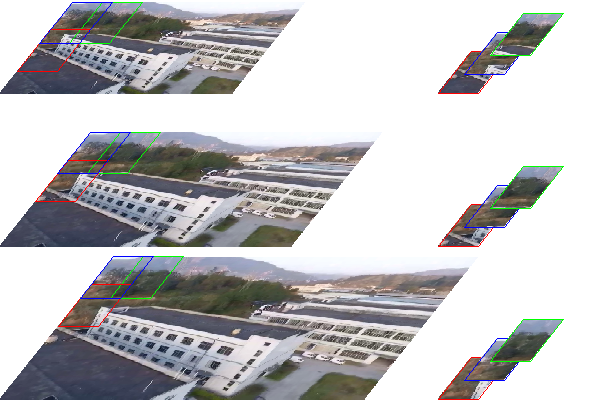
\includegraphics[width=0.9\linewidth]{images/piramid.png}
    \caption{Piramida obrazów wraz z~zaznaczonymi wybranymi oknami oraz wyekstrahowane okna przesuwne dla danej skali. Obraz pochodzi ze zbioru uczącego dostarczonego przez organizatorów konkursu \cite{dac_sdc_2021}.}
    \label{fig:sliding_window}
\end{figure}


Jednym z~często stosowanych podejść jest algorytm \emph{Viola-Jones}\cite{viola_jones}. 
Wykorzystywane jest tutaj okno przesuwne oraz tzw. cechy \emph{Haar}'a.
Reprezentują one układy jasności obrazu takie jak krawędzie, linie czy narożniki. 
Z obszaru definiowanego przez okno przesuwne ekstrahowane są cechy poddawane klasyfikacji metodą \emph{AdaBoost}.
Polega to na klasyfikacji z~użyciem kaskady tzw. słabych klasyfikatorów.
W przypadku, gdy jeden klasyfikator nie stwierdza wykrycia obiektu, pozostałe etapy klasyfikacji mogą zostać pominięte dla rozpatrywanego okna.
Obiekt jest uznawany za wykryty jedynie, gdy dla wszystkie klasyfikatory stwierdzą obecność obiektu. 

Innym przykładem może być podejście \emph{HOG}+\emph{SVM}\cite{hog} (ang. \emph{Histogram of Oriented Gradients + Support Vector Machine}). 
Wykorzystywany jest tutaj podział okna detekcji na komórki, w~których wyznaczane są histogramy orientacji gradientu. 
Histogramy są następnie normalizowane wewnątrz bloków składających się z~kilku komórek. 
Uzyskiwany jest wówczas wektor cech opisujący obszar obrazu wyznaczany przez okno przesuwne. 
Cechy te poddawane są klasyfikacji poprzez \emph{SVM}, której wynik daje informację o~obecności lub braku rozpatrywanego typu obiektu.

Metodą bazującą na cechach \emph{HOG} jest \emph{DPM} (ang. \emph{Deformable Part-based Model}) \cite{model_based}.
Podejście to bazuje na detekcji prostych obiektów, które składają się na obiekty o~większym stopniu skomplikowania.
Wykorzystywane jest tutaj dopasowanie modelów obiektów składowych do mapy cech \emph{HOG} (lub dowolnych innych).
Otrzymywane są w~ten sposób mapy prawdopodobieństwa wystąpienia danych klas.
Następnie wyniki te są analizowane poprzez mieszaninę modeli (ang. \emph{Mixture models}) obiektów złożonych.
Ponadto metoda ułatwia również detekcję obiektów deformowalnych tzn. mogących zmieniać kształt w~perspektywie czasu np. człowiek, u~którego położenie, orientacja i~kształt części ciała może się zmieniać w~czasie.


% Dokładność algorytmów wykorzystujących okno przesuwne jest zależna od kroku przesunięcia okna, a~także liczby rozpatrywanych skal. 
% Wykorzystanie wstępnej segmentacji może pozwolić osiągnąć  lepsze rezultaty, jednakże wymagane jest uzyskanie obrazu binarnego możliwego do uzyskania w~prostych przypadkach lub z~użyciem złożonych algorytmów. 

Wspomnie metody w~większości operują na technice okna przesuwnego, co ma wpływ na jakość detekcji.
Wykorzystywane są tutaj techniki klasyfikacji na podstawie wybranych cech reprezentujących zawartość okna.
Możliwa jest również detekcja poprzez wykorzystanie obrazu binarnego reprezentującego obiekt detekcji.
Stosując metody klasyczne zazwyczaj wymagany jest etap przetwarzania wstępnego składający się na filtrację, wyrównanie histogramu czy przekształcenia morfologiczne.


\section{Sieci neuronowe}

Dotychczas wymienione metody wymagały wcześniejszej ekstrakcji określonych cech bądź mapy segmentacji.
Stosując sztuczne sieci neuronowe (ang. \emph{Artificial Neural Networks}) możliwe jest połączenie etapów przetwarzania wstępnego, ekstrakcji cech, klasyfikacji jak również określenia położenia i~wymiarów obiektu. 
Pozwala to zarówno na względne uproszczenie systemu detekcji, lecz często również na osiągnięcie lepszych rezultatów. 
Odbywa się to jednak kosztem zwiększenia złożoności obliczeniowej oraz wymaga złożonego procesu uczenia z~użyciem dużych zbiorów danych.
W podrozdziale zostaną opisane wybrane metody detekcji wykorzystujące sieci neuronowe, a~także wybrane architektury z~przeznaczeniem sprzętowej implementacji.

\subsection{Wstęp do sztucznych sieci neuronowych}
Sztuczne sieci neuronowe stanowią algorytmy przetwarzania danych inspirowane biologicznymi procesami zachodzącymi w~układzie nerwowym \cite{SN_tadeusiewicz}. 
Wykorzystywane jest tutaj pojęcie tzw. sztucznego neuronu jako odpowiednika biologicznej komórki nerwowej. 
% Neurony stanowią główny element budulcowy sieci.
Neurony stanowią funkcje przetwarzające podane sygnały wejściowe oraz zwracające rezultat w~postaci sygnałów wyjściowych. 
Schemat neuronu przedstawiono na rysunku \ref{fig:neuron}.
Przedstawiony neuron realizuje operację iloczynu skalarnego pomiędzy wektorem wag $w$ oraz wektorem sygnałów wejściowych $x$ (wliczając stałą 1~stanowiącą sygnał bias).
Uzyskany rezultat jest najczęściej poddawany aktywacji wybraną funkcją nieliniową.
Większość neuronów posiada parametry zwane wagami. Mogą również zawierać elementy pamięci.
Neurony grupuje się w~tzw. warstwy (ang. \emph{layers}), które następnie odpowiednio łączy się ze sobą tworząc strukturę sztucznej sieci neuronowej (rysunek \ref{fig:net_schem}).
Dane wejściowe sieci są propagowane przez kolejne warstwy, aż do warstw stanowiących wyjść sieci.
Otrzymany rezultat jest zależny od parametrów neuronów poszczególnych warstw.

\begin{figure}
    \centering
    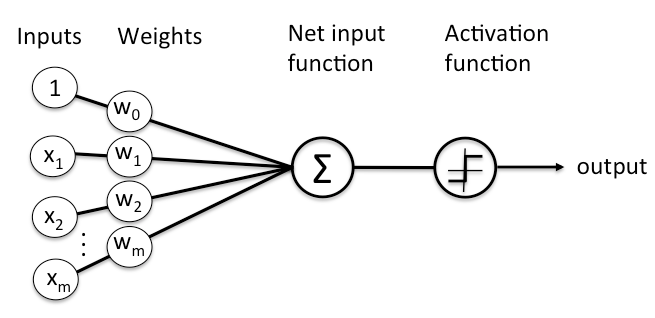
\includegraphics[width=0.6\linewidth]{images/neuron.png}
    \caption{Schemat neuronu. Źródło: \cite{neuron}.}
    \label{fig:neuron}
\end{figure}
\begin{figure}
    \centering
    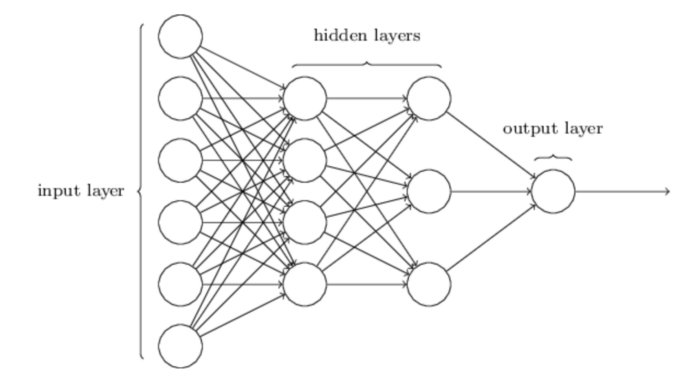
\includegraphics[width=0.6\linewidth]{images/net_schem.png}
    \caption{Schemat sieci neuronowej. Źródło: \cite{net_schem}.}
    \label{fig:net_schem}
\end{figure}

Sieć neuronowa posiada zdolność uczenia się tzn. zmian wartości parametrów na podstawie kolejno przedstawianych wzorców uczących wraz z~prezentowaniem referencyjnych rezultatów wyjściowych.
Proces ten nazywa się uczeniem sieci neuronowej.
Do tego celu definiuje się funkcję błędu wyjść, a~następnie odpowiednio aktualizuje się wagi z~wykorzystaniem tzw. propagacji wstecznej błędu.
Jednokrotne przedstawienie zbioru uczącego nazywane jest epoką, w~trakcie której następuje aktualizacja wag modelu sieci neuronowej.
Ponadto warstwy nie posiadające bezpośredniego połączenia z~wyjściem sieci nazywane są warstwami ukrytymi.
Sieć która posiada przynajmniej jedną warstwę ukrytą (realizującą operacje nielinowe) nazywana jest głęboką siecią neuronową (ang. \emph{Deep Neural Network}).
Sieć głęboka zyskuje zdolność wykształcania cech w~procesie uczenia przez warstwy ukryte. 
Każda kolejna warstwa ukryta wykształca bardziej ogólne cechy. 
Dokładniejsze omówienie sztucznych sieci neuronowych, nawiązanie do biologicznych odpowiedników, wybrane własności oraz metody uczenia można znaleźć \cite{SN_tadeusiewicz} oraz \cite{net_train}. 
Opisano tam przede wszystkim warstwy neuronów realizujących połączenia typu ``każdy z~każdym'', nazywane warstwami gęsto połączonymi (ang. \emph{Densly Connected}) lub w~pełni połączonymi (ang. \emph{Fully Connected}, \emph{FC}). 
Każdy neuron realizuje tam operacje iloczynu skalarnego wektora sygnałów wejściowych z~wektorem wag, niezależnie dla każdego neuronu.
% Ponadto warstwy te posiadają dużą skłonność do tzw. przeuczania, czyli nadmiernego dopasowywania (ang. \emph{overfitting}) do danych tracą zdolności generalizacji.

Zastosowanie głębokich sieci neuronowych wykorzystujących warstwy \emph{FC} dla problemów przetwarzania danych tego samego typu o~znacznych rozmiarach, takich jak obrazy (a także sygnały dźwiękowe, czy serie danych) skutkuje znaczącym rozbudowaniem architektury, wzrostem złożoności obliczeniowej, a~także trudnościami w~procesie uczenia. 
Możliwe jest wówczas zastosowanie tzw. konwolucyjnych sieci neuronowych (ang. \emph{Convolutional Neural Networks}, \emph{CNN}).
Definiują one sposób przetwarzania danych w~każdej warstwie w~sposób identyczny dla każdego neuronu wyznaczającego daną cechę.
Pozwala to na uproszczenie obliczeń, a~także na zwiększenie zdolności generalizowania danych.
Podstawą jest operacja konwolucji realizowana w~przestrzeni cech (lub obrazu dla warstwy wejściowej) z~wykorzystaniem maski konwolucji o~zadanym rozmiarze otoczenia oraz kształcie (elementy maski mogą zostać ``rozsunięte'' tzw. \emph{dilation}). 
Ponadto możliwe jest wykonanie operacji konwolucji z~krokiem większym od $1$, co skutkuje zmniejszeniem rozmiaru wynikowej mapy cech.
Za rodzaj wyznaczanych cech odpowiedzialny jest typ warstwy oraz ewentualne wagi filtrów. 
Wśród najczęściej stosowanych typów warstw konwolucyjnych wymienić można:
\begin{description}
\item warstwa konwolucyjna -- realizuje standardowe operacje konwolucji $Ch_{out}$ filtrami z~wagami dobieranymi w~procesie uczenia. Wymiary filtrów zależą od rozmiaru $(S_x,S_y)$ rozpatrywanego kontekstu oraz od liczby kanałów wejściowych $Ch_{in}$. 
\item warstwa próbkująca -- realizowane jest próbkowanie otoczenia definiowanego przez rozmiar maski.
Często stosowanymi są warstwy \emph{Max Pooling}, \emph{Min Pooling} czy \emph{Average Pooling} wykonujących kolejno operacje filtru maksymalnego, minimalnego oraz uśredniającego. Najczęściej przyjmowany jest krok konwolucji równy rozmiarowi maski, co skutkuje analizą niepokrywających się obszarów oraz redukcją wymiaru mapy cech.
\item warstwa normalizacyjna -- wykonywana jest operacja normalizacji kanałów wejściowych z~wykorzystaniem średniej kroczącej $\overline{x}_r$ oraz wariancji kroczącej $\sigma_r$, aktualizowanych w~trakcie przedstawiania kolejnych wzorców uczących zgrupowanych w~tzw. \emph{batch} .
Ponadto warstwa posiada dodatkowe wagi przekształcenia afinicznego $a, b$ wyznaczane w~procesie uczenia.
Równanie \eqref{eq:batch_norm} przedstawia wykonywaną operację dla danego kanału o~wartościach $x$ oraz dającej rezultat $y$. Ponadto wykorzystywana jest dodatkowa stała $\epsilon$ zapobiegająca dzieleniu przez $0$.  
\begin{equation}
y = a \frac{x-\overline{x}_r}{\sqrt{\sigma_r + \epsilon}} + b
\label{eq:batch_norm}
\end{equation}
\item warstwa aktywacji -- stanowi zastosowanie wybranej funkcji aktywacji np. $ReLU$, funkcji logistycznej czy \emph{softmax} ($sm$).
Często operacje aktywacji uznaje się jako realizowaną bezpośrednio w warstwie konwolucyjnej czy \emph{FC}.
\end{description}
Na rysunku \ref{fig:example_layers} przedstawiono przykładową architekturę sieci złożoną z~wybranych warstw konwolucyjnych oraz \emph{FC}. 
Wykorzystanie warstw \emph{FC} sprawia, iż wymagany jest stały rozmiar obrazu wejściowego.
W sytuacji gdy architektura sieci składa się tylko z~warstw konwolucyjnych rozmiar danych wejściowych jest niezależny od architektury. 
Architekturę taką nazywa się w~pełni konwolucyjną (ang. \emph{Fully Convolutional Neural Network}, \emph{FCNN}).
Warto również wspomnieć o~technice transferu wiedzy (ang. \emph{trasfer learning}). 
Polega ona na inicjalizacji wag wagami pochodzącymi od sieci już nauczonej (zazwyczaj na dużym zbiorze danych takim jak np. \emph{ImageNet}).
\begin{figure}
    \centering
    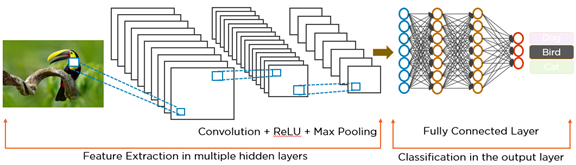
\includegraphics[width=0.9\linewidth]{images/layers_.png}
    \caption{Przykładowa architektura sieci \emph{CNN} wykorzystująca warstwy konwolucji, \emph{Max Pooling}, \emph{FC} oraz funkcje $ReLU$ przystosowane do zadania klasyfikacji obrazu.
    Źródło: \cite{layers_types}.}
    \label{fig:example_layers}
\end{figure}
 

\subsection{R-CNN}

We wcześniej wspomnianych metodach klasycznych wykorzystywano technikę okna przesuwnego oraz skalowanie obrazu. 
W metodzie \emph{R-CNN} (ang. \emph{Regions with CNN features}) \cite{r_cnn} analizowane są jedynie wybrane regiony obrazu. 
Wybór regionów jest dokonywany za pomocą wybranego algorytmu np. przeszukiwania selektywnego (ang. \emph{Selective Search}) \cite{sel_search}.
Następny etap polega na ekstrakcji cech z~uzyskanych wcześniej obszarów.
Wymagane jest aby wektory cech posiadały ustalony rozmiar. 
Z tego powodu proponowane obszary są skalowane do ustalonego rozmiaru.
Ekstrakcja cech odbywa się z~użyciem przetrenowanej (np. na zbiorze \cite{imagenet}) sieci CNN.
Możliwe jest wykorzystanie dowolnych architektur CNN np. \emph{AlexNet} \cite{alexnet}, \emph{VGG-16} \cite{vgg}.
Ostatni etap to klasyfikacja oraz regresja.
W tym celu należy przeprowadzić trening dowolnego klasyfikatora np. sieć \emph{FC} lub \emph{SVM} stwierdzającego obecność lub brak rozpatrywanego typu obiektu w~rozpatrywanym obszarze.
W przypadku wykrycia obiektu znane są jego przybliżone położenie oraz wymiary.
Celem zwiększenia dokładności detekcji dokonywane są estymaty położenia i~wymiarów, poprzez regresję liniową.

Etap ekstrakcji cech wymagał przetworzenia każdego obszaru obrazu przez całą sieć.
Możliwe jest również wstępne przetworzenie całego obrazu tylko przez warstwy konwolucyjne.
Uzyskiwane są w~ten sposób mapy cech dla całego obrazu.
Następnie fragmenty map odpowiadające wejściowym proponowanym regionom, po odpowiednim przeskalowaniu do ustalonego wymiaru, poddawane są klasyfikacji oraz regresji parametrów.
Do tego celu używana jest sieci neuronowa wykorzystująca warstwy \emph{FC}.
Pozwala to na zwiększenie szybkości działania systemu.
Wspomniane rozwinięcie metody nazywane jest \emph{Fast R-CNN} \cite{fast_rcnn}.

Obie wspomniane metody bazowały na proponowanych poprzez wybrany algorytm regionach obrazu.
Etap ten można zastąpić użyciem do tego celu wytrenowanej sieci neuronowej nazywanej \emph{Region Proposal Network} (RPN).
Ponadto sieć ta może bazować na mapach cech wykorzystywanych do ekstrakcji wektorów cech stałowymiarowych  dla proponowanych regionów. 
Rozwiązanie to nazywane jest \emph{Faster R-CNN} \cite{faster_rcnn}.
\begin{figure}
    \centering
    \begin{subfigure}[b]{0.48\textwidth}
         \centering
         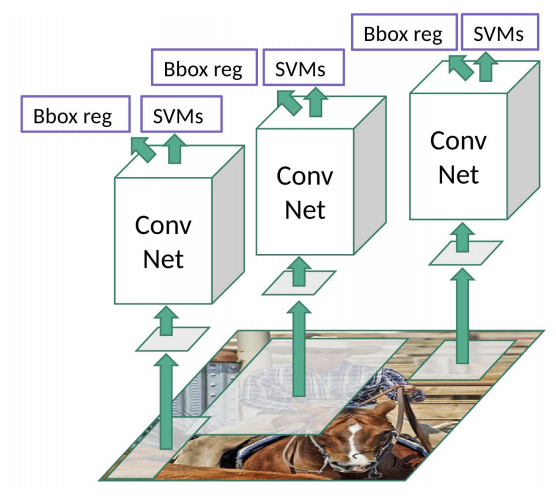
\includegraphics[width=\textwidth]{images/rcnn.png}
         \caption{}
         \label{fig:rcnn}
     \end{subfigure}
     \hfill
    \begin{subfigure}[b]{0.48\textwidth}
         \centering
         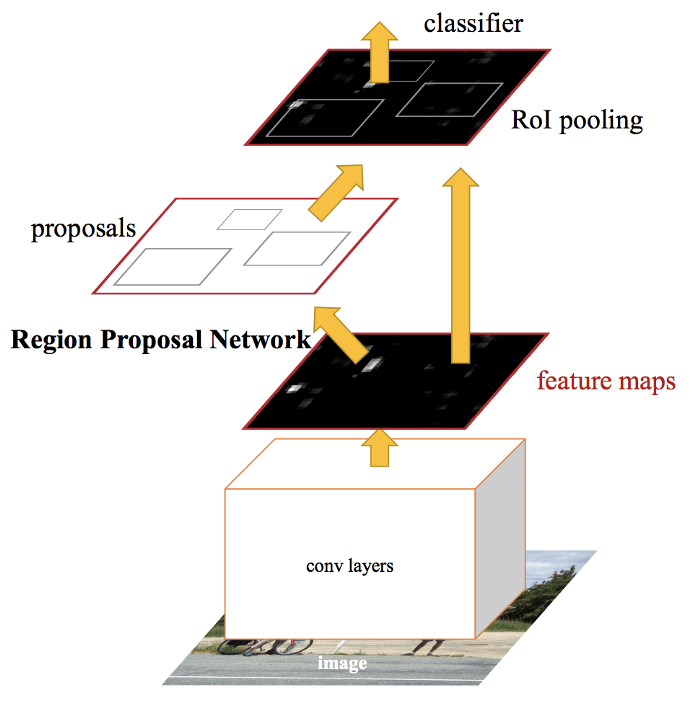
\includegraphics[width=\textwidth]{images/ffrcnn.png}
         \caption{}
         \label{fig:ffrcnn}
     \end{subfigure}
     \hfill
    \begin{subfigure}[b]{0.9\textwidth}
         \centering
         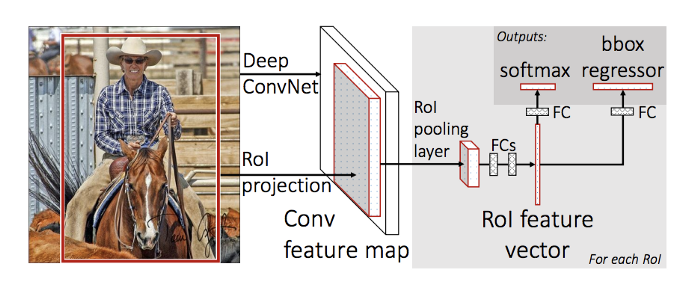
\includegraphics[width=0.8\textwidth]{images/frcnn.png}
         \caption{}
         \label{fig:frcnn}
     \end{subfigure}
     \hfill
    \caption{Architektury \emph{R-CNN} \ref{fig:rcnn}, \emph{Faster R-CNN} \ref{fig:ffrcnn} oraz \emph{Fast R-CNN} \ref{fig:frcnn}. Źródło: \cite{medium_rcnn}.}
    \label{fig:rcnns}
\end{figure}

\subsection{SSD}
Systemy detekcji bazujące na rozwiązaniu \emph{R-CNN} wymagają dwuetapowego przetwarzania obrazu.
W architekturze \emph{Single Shot Detector} (SSD) \cite{ssd} detekcja obiektów wykonywana jest jednoetapowo.
Wykorzystywana do tego celu jest jednokierunkowa sieć w~pełni konwolucyjna (ang. \emph{Fully Convolutional Neural Network},\emph{FCNN}) stanowiąca tzw. sieć bazową (ang. \emph{base network}) przetrenowaną do zadania klasyfikacji (bez "głowy" klasyfikatora).
Za ostatnią warstwą sieci bazowej dołączane są dodatkowe warstwy konwloucyjne oraz \emph{Max pooling} celem zmniejszenia rozmiaru map cech.
Do wybranych warstw pośrednich przyłączane są kolejne warstwy tworząc rozgałęzienia.
Każde rozgałęzienie zakończone jest warstwą konwolucyjną, której filtry realizują zadania klasyfikacji wykrycia obiektu, typu oraz regresji jego parametrów. 
Na rysunku \ref{fig:ssd_arch} przedstawiono architekturę \emph{SSD}, gdzie jako sieć bazową wykorzystano \emph{VGG-16}. 
Estymacja wymiarów odbywa się względem ustalonych wymiarów $(d_w, d_h)$ nazywanych \emph{default box} (dla każdego zastawu filtrów detekcja + klasyfikacja może zostać dobrany inny wymiar $(d_w, d_h)$).
Położenie obiektu jest wyznaczane w~oparciu o~rezultaty odpowiednich filtrów ($f_x, f_y, f_w, f_h$), lecz także o~ich położenie $(i,j)$ w~siatce (ang. \emph{grid}) wynikającej z~wymiarów warstwy $(d_N, d_M)$ znormalizowane do wymiarów \emph{default box}.
Ostatecznie detekcja parametrów obiektu daje się przedstawić za pomocą równań \eqref{eq:xs_ssd}-\eqref{eq:h_ssd} ($(W, H)$ oznaczają wymiary obrazu wejściowego). 

\begin{figure}
    \centering
    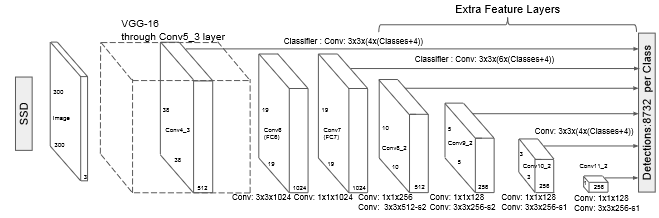
\includegraphics[width=0.9\linewidth]{images/ssd_img.png}
    \caption{Architektura \emph{SSD}. Do sieci bazowej dołączone są kolejne warstwy wraz rozgałęzieniami.
    Źródło \cite{ssd}.}
    \label{fig:ssd_arch}
\end{figure}
\begin{figure}
    \centering
    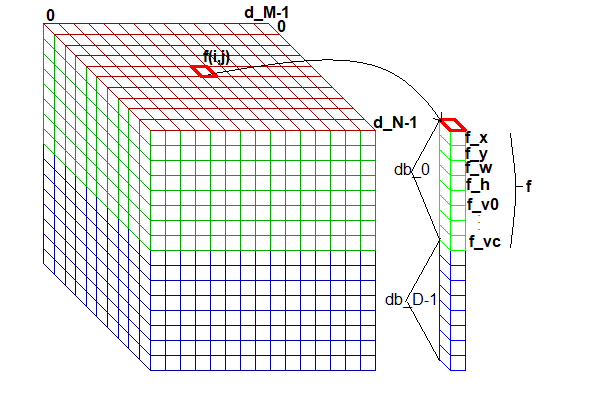
\includegraphics[width=0.9\linewidth]{images/ssd_grid_marked.png}
    \caption{Siatka detekcji dla $D$ \emph{default box}. Poprzez $db$ oznaczono grupę filtrów przypisanych do konkretnego \emph{defult box}. Filtry $v0,...vc$ oznaczają kolejne klasy obiektów.}
    \label{fig:ssd_grid}
\end{figure}

\begin{equation}
x_s = (\frac{j}{d_N}+ 0.5)W + d_w f_x(i,j)
\label{eq:xs_ssd}
\end{equation}
\begin{equation}
y_s = (\frac{i}{d_M}+ 0.5)H + d_h f_y(i,j)
\label{eq:ys_ssd}
\end{equation}
\begin{equation}
w = d_we^{f_w(i,j)}
\label{eq:w_ssd}
\end{equation}
\begin{equation}
h = d_he^{f_h(i,j)}
\label{eq:h_ssd}
\end{equation}

Trening sieci odbywa się w~oparciu o~sumę błędu klasyfikacji oraz błędu regresji.
Błąd regresji $L_{reg}$ jest reprezentowany przez sumę błędów bezwzględnych znormalizowanego przesunięcia względem środka w~siatce oraz wykładnika eksponencjalnego przeskalowania względem wymiarów \emph{default box}. 
Równanie \eqref{eq:loss_reg_ssd} przedstawia funkcję błędu dla pojedynczego \emph{default box} dla referencyjnych parametrów $i, j, x_{ref}, y_{ref}, w_{ref}$ oraz $h_{ref}$.
Poprzez $f$ oznaczono rezultaty filtracji wcześniej wspomnianymi filtrami.
\begin{equation}
\begin{aligned}
L_{reg}(f, d, i, j, x_{ref}, y_{ref}, w_{ref}, h_{ref}) 
=& |f_x(i,j) - \frac{x_{ref}\frac{d_N}{W} - j - 0.5}{d_w}| \\
&+ |f_y(i,j) - \frac{y_{ref}\frac{d_M}{H} - i - 0.5}{d_h}| \\
&+ |f_w(i,j) - log(\frac{w_{ref}}{d_w})|\\
&+ |f_h(i,j) - log(\frac{h_{ref}}{d_h})|
\end{aligned}
\label{eq:loss_reg_ssd}
\end{equation}

Błąd klasyfikacji $L_{class}$ jest obliczany przy pomocy funkcji danej wzorem \eqref{eq:loss_class_ssd}. Poprzez $f$ oznaczono zbiór filtrów realizujących zadanie klasyfikacji, $C$ oznacza referencyjną mapę klas dla danego \emph{default box} $d$, gdzie każdy element mapy oznacza numer klasy. Należy zauważyć, iż dla elementów, dla których nie powinno nastąpić wykrycie, również przypisana jest klasa oznaczająca brak wykrycia obiektu.

\begin{equation}
L_{class}(f,d,C) = 
-\sum_{ii}^{d_M}{\sum_{jj}^{d_N}
{log(sm(f_{v}))_{C(ii,jj)}(ii,jj)}
}
\label{eq:loss_class_ssd}
\end{equation}


Przedstawione równania stanowią składowe błędu całej sieci $L$, przy czym są one sumowane dla każdego \emph{default box} oraz dla każdego zestawu parametrów referencyjnych.
W równaniu \eqref{eq:total_SSD} poprzez $D$ oznaczono zbiór \emph{default box} $d$. 
Przyjmując za do $dd$ jako wybrany \emph{default box},  $f^dd$ stanowi zestaw filtrów przypisanych $dd$, $C^dd$ jest maską referencyjną klas dla $dd$. 
Poprzez $R$ oznaczono zbiór parametrów referencyjnych $r$ opisujących dany obiekt.
\begin{equation}
    L(f, D, C, R) = \sum_{d \in D} {L_{class}(f^d,d,C^d)} + \sum_{r \in R}{L_{reg}(f^{r_d},r_d,r_i,r_j,r_x,r_y,r_w,r_h)}
\label{eq:total_SSD}
\end{equation}

W przedstawionych równaniach filtr wykrycia obiektu nie występuje jawnie, lecz pod postacią klasy ``niewykrycia obiektu''. 
Architektura \emph{SSD} znacząco upraszcza implementację zadania detekcji, poprzez jednoetapowe przetwarzanie obrazu. 


\subsection{YOLO}
\label{ch:yolo}
Poprzednikiem architektury \emph{SSD} w~detekcji jednoetapowej była architektura YOLOv1 (ang. \emph{You Only Look Ones}) \cite{yolov1}.
Architektura ta wykorzystywała podział obrazu na siatkę o~określonych wymiarach odpowiadających wymiarom ostatniej warstwy typu \emph{Fully Connected} (\emph{FC}).
W przypadku architektury \emph{SSD} kolejne filtry stanowiły klasyfikację oraz regresję, 
dla \emph{YOLOv1} tę rolę spełniają odpowiednie neurony warstwy \emph{FC} poprzez stosowną interpretację dla wymiaru $BxSxSx(5+C)$, gdzie $B$ to liczba estymowanych \emph{bounding box}, $S$ wymiar siatki, $C$ liczba rozpatrywanych klas. 
Stała wartość $5$ oznacza liczbę neuronów spełniających rolę wykrycia obiektu oraz estymacji parametrów obiektu.
Trening architektury sprowadzał się do minimalizacji ważonej sumy kwadratów błędów dla położenia, błędów pierwiastków wymiarów, błędów klasy oraz błędów wykrycia obiektu. 
Ponadto błędy te były wyznaczane tylko dla elementów siatki, w~których występował (częściowo lub w~pełni) obiekt referencyjny.
Na rysunku \ref{fig:yolo_img} zilustrowano metodę detekcji opartą o~architekturę \emph{YOLO}.

\begin{figure}
    \centering
    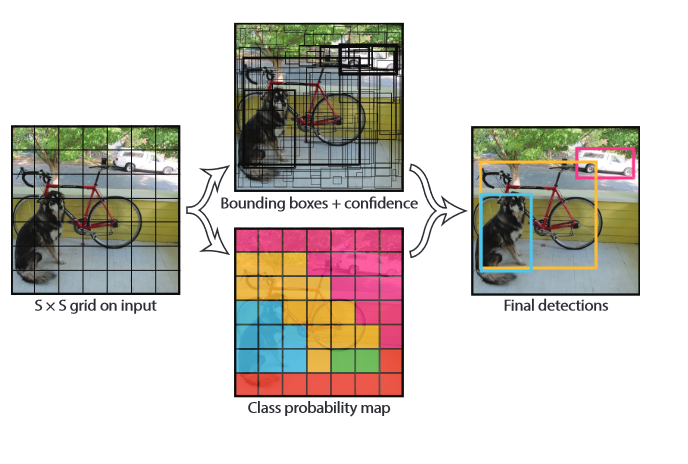
\includegraphics[width=0.9\linewidth]{images/yolo.png}
    \caption{Metoda detekcji oparta o~architekturę \emph{YOLO}. Źródło: \cite{yolov1}}
    \label{fig:yolo_img}
\end{figure}

Wykorzystanie warstw \emph{FC} w~\emph{YOLOv1} uniemożliwiło realizację przetwarzania w~wielu skalach.
% Warstwa ta nie występuje w~\emph{SSD}.
Z tego powodu w~następnych wersjach YOLOv2 \cite{yolov2} oraz YOLOv3 \cite{yolov3} również odrzucono warstwę \emph{FC} na rzecz warstw konwolucyjnych z~filtrami $f$ o~wymiarach 1x1 uzyskując architekturę \emph{FCNN}. 
Wyznaczenie parametrów obiektów zostało przedstawione poprzez równania \eqref{eq:xc_yolov2}-\eqref{eq:h_yolov2}. Poprzez $(a_w,a_h)$ oznaczono wymiary tzw. \emph{anchor box}, stanowiącego odpowiednik \emph{default box} w~\emph{SSD}. 
Wymiary siatki oznaczono poprzez $(a_N,a_M)$. Natomiast $(a_x,a_y)$ oznaczają położenie indeksy elementu siatki, dla którego wyznaczane są parametry. 
\begin{equation}
x_c = (\sigma(f_x) + a_x) \frac{W}{a_N}
\label{eq:xc_yolov2}
\end{equation}
\begin{equation}
y_c = (\sigma(f_y) + a_y) \frac{H}{a_M}
\label{eq:yc_yolov2}
\end{equation}
\begin{equation}
w = a_w e^{f_w}
\label{eq:w_yolov2}
\end{equation}
\begin{equation}
h = a_h e^{f_h}
\label{eq:h_yolov2}
\end{equation}
Zastosowanie funkcji logistycznej w~estymacji położenia pozwala na osiągnięcie większej stabilności regresji \cite{yolov2}, czy korelacji pomiędzy wykryciem obiektu w~siatce, a~predykcją jego położenia.
Linowa estymacja odchyłki położenia pozwalała  na ''przesunięcie'' obiektu do elementu siatki o~niskiej wartości wykrycia. 
Wiązało by się to co najmniej z~brakiem spójności pomiędzy wykryciem obiektu, a~jego położeniem.
Powodem tego był brak ograniczenia przyjmowanych wartości poszczególnych neuronów. 
Ponadto referencyjne wartości wykrywalności obiektu dla \emph{YOLOv2} stanowią wartość współczynnika $IoU$ pomiędzy obiektem referencyjnym, a~rozpatrywanym \emph{anchor box} (stanowiącym odpowiednik \emph{default box} w~\emph{SSD}). 
Dla \emph{YOLOv3} wykrywalność obiektu (autorzy używają sformułowania \emph{objectness score} \cite{yolov3}) jest zrealizowana jako regresja logistyczna. 
Z tego powodu wartości referencyjne przyjmują wartość $1$ w~przypadku, gdy wartość $IoU$ jest większa niż ustalona wartość progowa oraz $0$ w~przeciwnym przypadku. 

Kolejna wersja \emph{YOLOv4}\cite{yolov4} znacząco poprawia rezultaty względem wersji poprzednich, lecz jest również znacznie bardziej skomplikowana. Trening \emph{YOLOv3} zakładał minimalizację sumy kwadratów błędów dla części regresyjnej. W~wersji \emph{YOLOv4} autorzy\cite{yolov4} zalecają użycie funkcji błędu reprezentowanej przez \emph{CIoU} \cite{dciou} danej równaniem \eqref{eq:ciou}.
Wspomniane są również inne funkcje bazujące na metryce \emph{IoU} takie jak \emph{GIoU}\cite{giou} \eqref{eq:giou} oraz \emph{DIoU} \cite{dciou} \eqref{eq:diou}.

\begin{equation}
GIoU(A,B) = 1 - IoU(A,B) + giou_{part}(A,B)
\label{eq:giou}
\end{equation}
\begin{equation}
DIoU(A,B) = 1 - IoU(A,B) + diou_{part}(A,B)
\label{eq:diou}
\end{equation}
\begin{equation}
CIoU(A,B) = 1 - IoU(A,B) + diou_{part}(A,B) + ciou_{part}(A,B)
\label{eq:ciou}
\end{equation}

\begin{equation}
giou_{part}(A,B) = \frac{|C \setminus (A \cup B)|}{|C|}
\label{eq:giou_part}
\end{equation}
\begin{equation}
diou_{part}(A,B) = \frac{(A_{x_c} - B_{x_c})^2 + (A_{y_c} - B_{y_c})^2}{C_w^2+C_h^2}
\label{eq:diou_part}
\end{equation}
\begin{equation}
v(A,B) = \frac{4}{\pi^2} (arctan(\frac{A_w}{A_h}) - arctan(\frac{B_w}{B_h}))^2
\label{eq:ciou_v}
\end{equation}
\begin{equation}
\alpha(A,B) = \frac{v(A,B)}{1 - IoU(A,B) + v(A,B)}
\label{eq:ciou_alpha}
\end{equation}
\begin{equation}
ciou_{part}(A,B) = \alpha(A,B) v(A,B)
\label{eq:ciou_part}
\end{equation}


Oznaczenia:
\begin{description}
\item $A, B, C$ -- \emph{bounding box}
\item $C$ -- najmniejszy \emph{bounding box} taki, że $A,B \subseteq C$
\end{description}

Analizując powyższe wzory można dostrzec, iż gdy:
\begin{itemize}
\item obiekty nie posiadają  części wspólnej $IoU = 0$,
\item obiekty zawierają się w~sobie $giou_{part} = 0$,
\item środek obiektów znajduje się w~tym samym punkcie $diou_{part} = 0$,  
\item $ciou_{part}$ ma wpływ tylko na błąd wynikający z~wymiarów obiektu. 
\item $ciou_{part}$ dla obiektów o~tym samym stosunku wymiarów, lecz o~różnych wymiarach przybiera wartość $0$. 
\end{itemize}

Funkcja $DIoU$ minimalizuje odstęp pomiędzy obiektami, $CIoU$ rozwija tę funkcję o~skalowanie wymiarów, natomiast $GIoU$ pozwala na ograniczenie obszaru poza obiektami referencyjnym oraz wyznaczonym z~odpowiedzi sieci.
Na rysunku \ref{fig:iou_losses} przedstawiono graficzne interpretacje błędów.

\begin{figure}
    \centering
     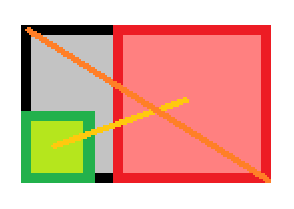
\includegraphics[width=0.4\linewidth]{images/gcdiou.png}
    \caption{ Graficzna reprezentacja $GIoU$, $DIoU$ dla obiektów $A$(czerwony)  oraz $B$ (zielony) o~tym samym stosunku wymiarów ($ciou_{part} = 0$).
    Poprzez $C$ (czarny) oznaczono najmniejszy \emph{bounding box} zawierający obiekty $A$ i $B$.
    $diou_{parts}$ to stosunek długości linii żółtej do pomarańczowej. 
    $giou_{part}$ to stosunek szarego pola powierzchni ($C \setminus (A\cupB)$) do pola powierzchni$C$.}
    \label{fig:iou_losses}
\end{figure}

\section{Przegląd rozwiązań energooszczędnych}

Dotychczas omawiane metody detekcji nie były projektowane z~myślą o~optymalizacji zużycia energii czy łatwości implementacji sprzętowej. 
Ze względu na to, iż celem konkursu DAC SDC 2021 jest sprzętowa implementacja w~układzie FPGA, warto również rozpatrzyć rozwiązania pozwalające nie tylko osiągnąć wysoką, dokładność, lecz również zmniejszyć zużycie energii i~zwiększyć przepustowość.

\subsection{Konwolucja separowalna}
\label{subsec:sep_conv}

Jednym z~częstych rozwiązań przeznaczonych dla urządzeń mobilnych o~małej mocy obliczeniowej jest zastosowanie konwolucji separowalnych (ang. \emph{Separable Convolution}). 
Wykonywane są tu kolejno po sobie dwa typy konwolucji \emph{Depthwise} (\emph{DW}) oraz \emph{Pointwise} (\emph{PW}). 
Konwolucja \emph{DW} polega na niezależnej filtracji poszczególnych kanałów (głębi) (podobnie jak ma to miejsce w~przypadku konwolucji dla obrazu w~skali szarości).
Maska konwolucji \emph{DW} posiada jedynie dwa wymiary przez co możliwa jest analiza kontekstu jedynie w~obrębie jednego kanału.
Konwolucja \emph{PW} stanowi szczególny przypadek pełnej konwolucji (standardowej) z~filtrem o~wymiarach 1x1 (stosowanym np. w~warstwach \emph{YOLO}).
Pozwala to uprościć obliczenia ze względu na brak analizowania kontekstu / otoczenia rozpatrywanego punktu (ang. \emph{point}) maski cech.
Maska konwolucji \emph{PW} posiada jeden wymiar równy liczbie kanałów wejściowych.
Połączenie obu konwolucji pozwala na aproksymację pełnej konwolucji zachowując własność analizy kontekstu pomiędzy kanałami, przy zmniejszeniu liczby obliczeń. 
Ponadto po konwolucji \emph{DW} możliwe jest zastosowanie dodatkowych nieliniowości.
Pierwszą architekturą, w~której zastosowanie konwolucji separowalnych przyniosło olbrzymi sukces był \emph{GoogLeNet}\cite{inception_googlenet}. 
Dla zastosowań mobilnych tego typu konwolucje zostały wprowadzone w~architekturze \emph{MobileNet}\cite{mobilenet}. 
Zastosowanie konwolucji separowalnych pozwala zarówno na ograniczenie pamięci wymaganej na przechowywanie modelu, jak również na zmniejszenie liczby wymaganych obliczeń.
Rysunki \ref{fig:dw} oraz \ref{fig:pw} przedstawiają schemat konwolucji \emph{DW} oraz \emph{PW}. 

\begin{figure}
    \centering
    \hfill
    \begin{subfigure}[b]{0.98\textwidth}
    \centering
    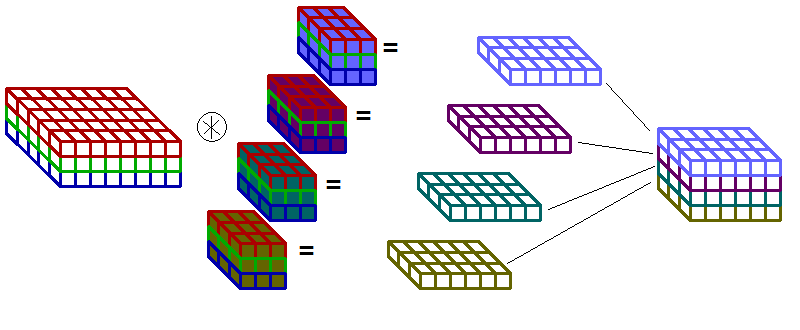
\includegraphics[width=\textwidth]{images/std_conv.png}
    \caption{}
    \label{fig:std_conv}
    \end{subfigure}
    \hfill
    \begin{subfigure}[b]{0.98\textwidth}
    \centering
    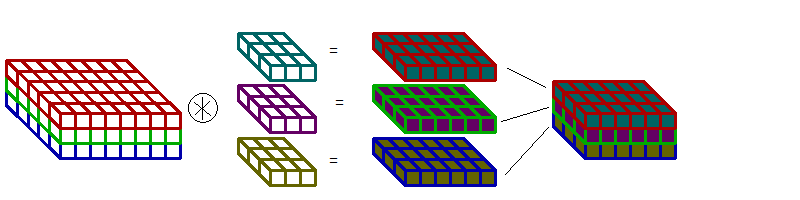
\includegraphics[width=\textwidth]{images/dw_conv.png}
    \caption{}
    \label{fig:dw}
    \end{subfigure}
    \hfill
    \begin{subfigure}[b]{0.98\textwidth}
    \centering
    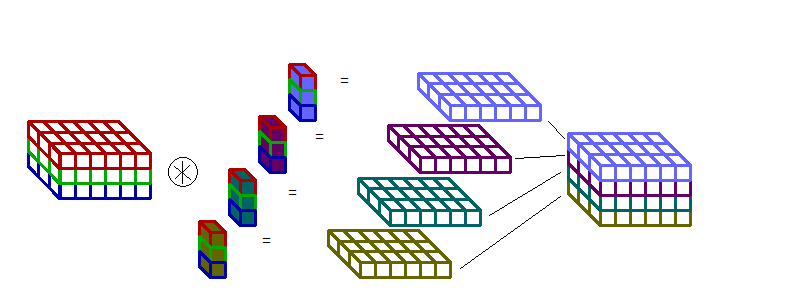
\includegraphics[width=\textwidth]{images/pw_conv.png}
    \caption{}
    \label{fig:pw}
    \end{subfigure}
    
    \caption{Schemat konwolucji pełnej\ref{fig:std_conv}, \emph{depthwise} \ref{fig:dw} oraz \emph{pointwise} \ref{fig:pw}.}
    \label{fig:dw_pw_schema}
\end{figure}

\subsection{Sieci kwantyzowane}
Obliczenia zmiennoprzecinkowe pozwalają na osiągnięcie wysokiej dokładności obliczeń wraz z~szerokim zakresem zmienności.
Czas obliczeń zmiennoprzecinkowych jest zazwyczaj dłuższy w~porównaniu do obliczeń całkowitoliczbowych.
Algorytmy sieci neuronowych w~większości przypadków są projektowane do implementacji z~wykorzystaniem wspomnianego typu obliczeń. 
Jednakże nie zawsze wymagana jest wysoka precyzja obliczeń.
Wówczas możliwe jest zastosowanie tzw. kwantyzowanych sieci neuronowych (ang. \emph{Quantized Neural Networks}, \emph{QNN}) \cite{qnn} możliwych do implementacji z~wykorzystaniem obliczeń całkowitoliczbowych (ang. \emph{integer}) czy stałoprzecinkowych (ang. \emph{fixedpoint}).
Aby jednak możliwa była tak implementacja wymagane jest przeprowadzeniu kwantyzacji.
Proces polega na odpowiednim przetransformowaniu wag oraz wyników pośrednich tak, aby odwzorować obliczenia o~ograniczonej precyzji.
Równanie \eqref{eq:quant} przedstawia kwantyzację stałoprzecinkową.
Funkcja $Q$ wykonuje operację kwantyzacji stałoprzecinkowej zmiennej zmiennoprzecinkowej $x$, dla zapisu na $b$ bitach z~bitem znaku ($s=1$) lub bez ($s=0$), przy wykorzystaniu $i$ bitów na część całkowitą i~znak oraz z~metodą przybliżenia do liczby całkowitej $n$.
\begin{equation}
min_{int}(b,s) = -s 2^{b-s}
\end{equation}
\begin{equation}
max_{int}(b,s) = 2^{b-s}-1
\end{equation}
\begin{equation}
limit(x_{int},b,s) = \min(\max(x,min_{int}(b,s)),max_{int}(b,s))
\end{equation}
\begin{equation}
scale(b,i) = \frac{1}{2^{b-i}}
\end{equation}
\begin{equation}
int(x,b,i,s,n) = limit(n(\frac{x}{scale(b,i)}), b,s)
\label{eq:to_int}
\end{equation}
\begin{equation}
Q(x,b,i,s,n) = int(x,b,i,s,n) \ scale(b,i)
\label{eq:quant}
\end{equation}

Funkcja $Q$ zwraca rezultat w~postaci przybliżenia do liczby stałoprzecinkowej.
Jako metody przybliżenia możliwe jest użycie zaokrąglenia w~dół (podłoga, ang. \emph{floor}), w~górę (sufit, ang. \emph{ceil}) lub do najbliższej wartości całkowitej (ang. \emph{round}).
Model sieci z~przeprowadzoną kwantyzacją wymaga dalszego uczenia, ze względu możliwą utratę dokładności lub ograniczenie wartości do zakresu liczb stałoprzecinkowych.
Uzyskanie zapisu z~wykorzystaniem liczb całkowitych (celem ewaluacji sprzętowej lub programowej modelu) jest możliwe poprzez równanie \eqref{eq:to_int}.

\subsection{Sieci binarne}

Przedstawiona dotychczas kwantyzacja wykorzystywała więcej niż 1 bit do zapisu danych.
Przy kwantyzacji 1 bitowej uzyskiwana jest tzw. binarna sieć neuronowa (ang. \emph{Binary Neural Network}, \emph{BNN}) \cite{qnn}.
W sieciach binarnych odpowiednikiem operacji mnożenia jest operacja $xnor$, natomiast sumowania operacja zliczania bitów. 
Aby dokonać kwantyzacji binarnej $Q_b$ zmiennej $x$ wykorzystuje się funkcję $sign$. 
Otrzymywana wartość pochodzi ze zbioru $\{-1,1\}$.
\begin{equation}
Q_b(x) = sign(x)
\label{eq:binarize}
\end{equation}
Kwantyzację binarną można również zrealizować w~sposób stochastyczny\cite{qnn}.
Przedstawiono poprzez równanie \eqref{eq:stochastic}. 
Poprzez $r$ oznaczono zmienną losową z~przedziału $[0;1]$. 
Funkcja $\sigma_h$ oznacza funkcję \emph{hard sigmoid}.
\begin{equation}
Q_{bs}(x) =
\begin{cases}
1 & r < \sigma_h(x) \\
-1 & otherwise
\end{cases}
\label{eq:stochastic}
\end{equation}

Celem dalszego procesu uczenia wykorzystuje się dodatkowy parametr skalujący rezultat kwantyzacji uzyskiwany w~sposób analityczny \cite{xnor_net} lub stanowiący jeden z~parametrów procesu uczenia \cite{xnor_net++}.
Dodatkowo w~\cite{qnn} zaleca się ograniczenie wartości wag i~wyników pośrednich do przedziału $[-1;1]$

Sieci binarne pozwalają na znaczą redukcję pamięci potrzebnej do przechowywania wag, a~także znacząco upraszczają obliczenia.

\subsection{Ultra\_net}

Mając na uwadze iż jednym z~warunków konkursu jest udostępnienie pełnego rozwiązania w~formie otwarto-źródłowej, możliwa jest analiza rozwiązań z~edycji poprzedzających rozpatrywaną.
Zwycięski zespół poprzedniej edycji (2020) wykorzystał architekturę sieci \emph{Ultra\_net} \cite{ultra_net}. 
Jest to architektura \emph{FCNN} zawierająca 9 warstw kowolucyjnych, warstwy normalizujące, warstwy \textit{Max Pooling} oraz warstwę \emph{YOLOv3} \cite{yolov3}.
Ponadto warstwy konwolucyjne zawierały co najwyżej 64 filtry o~wymiarach kontekstu 3x3.
Sprzętowa akceleracja została zrealizowana z~użyciem języka \emph{HLS} (ang. \emph{High Level Synthesis}). 
Wykorzystano tutaj 4 bitową kwanytyzację wag konwolucji. 
Dla warstw normalizacyjnych kwantyzacja była zmienna (stała dla warstwy, lecz zależna od jej  położenia).
Rozwiązanie osiągnęło dokładność detekcji $0.656$ współczynnika \emph{IoU}, przepustowość $212.726 fps$ oraz zużyło $1641.1 J$ energii. 

\subsection{SkyNet}
Innym rozwiązaniem jest architektura \emph{SkyNet} \cite{skynet}. 
Przez 3 ostatnie edycje architektura ta osiągała jedne z~najlepszych wyników.
Jest to również sieć typu \emph{FCNN}, wyróżniająca się zastosowaniem konwolucji seperowalnych oraz funkcji aktywacji $ReLU6$.
W każdym bloku konwolucji separowalnej, po każdej warstwie konwolucji \emph{DW} oraz p\emph{PW}  występuje warstwa normalizacji z~funkcją aktywacji.
Ostatnią warstwę sieci stanowi warstwa \emph{YOLOv3} (podobnie jak w~przypadku \emph{Ultra\_net}).
Liczba filtrów w~warstwach oraz położenie warstw \textit{Max Pooling} zostały zoptymalizowane z~użyciem algorytmu \emph{PSO} (ang. \emph{Particle Swarm Optimization}).
Implementacja została zrealizowana z~użyciem języka \emph{HLS}.
Wykorzystano tutaj dwa akceleratory - po jednym dla każdego typu konwolucji.
Każda kolejna warstwa była obliczana sekwencyjnie tzn. w~jednej chwili czasu obliczana była tylko jedna warstwa.  
Rozwiązanie osiągnęło dokładność detekcji $0.716$ IoU, przepustowość $25.05 fps$ oraz zużyło $7260 J$ energii dla implementacji na płytce \emph{Avnet Ultra96 V1}. 

Architektura \emph{SkyNet} osiąga lepszą jakość detekcji, niż architektura \emph{Ultra\_net}. 
Jednakże zrealizowana implementacja charakteryzuje się stosunkowo niską przepustowością oraz wysokim zużyciem energii.

% \subsection{XNOR-Net}

% Dotychczas przytoczone rozwiązania wykorzystywały sieci z~kwantyzacją wielobitową oraz pochodzące z~poprzednich edycji konkursu. 
% Innym podejściem mogącym uzyskać zwiększoną przepustowość oraz mniejsze zużycie energii jest zastosowanie sieci binarnych.
% Przykładem jest sieć \emph{XNOR-Net}\cite{xnor_net}. 
% Wagi oraz wejścia warstw sieci są poddawane binaryzacji funkcją \eqref{eq:binarize}.
% Binarne wartości poddawane są binarnej konwolucji, która różni się względem standardowej użyciem funkcji $xnor$ zamiast mnożenia oraz zliczania bitów w~miejsce sumowania0.
% Zastosowanie kwantyzacji binarnej znacząco zmienia uzyskiwane wyniki (tych samych operacji) w~stosunku do modelu przed binaryzacją.
% Celem zmniejszenia różnicy rezultatów wprowadzono współczynniki skalujące wyznaczane analitycznie. 
% Następcą sieci \emph{XNOR-Net} jest sieć \emph{XNOR-Net++}\cite{xnor_net++}. 
% W~sieci tej zastąpiono wyznaczane analitycznie współczynniki na rzecz dodatkowych parametrów sieci wyznaczanych w~trakcie wstecznej propagacji błędu.
% Obie wspomniane sieci binarne były testowane przez autorów dla zadania klasyfikacji. 
% Jednakże opisana metodyka może również być zastosowana dla zadania detekcji.

% podsumowanie
Zadanie detekcji sprowadza się do znalezienia położenia obiektu oraz jego wymiarów, a~często również określenia typu obiektu (klasyfikacja). 
Rozwiązanie problemu możliwe jest z~wykorzystaniem zarówno metod klasycznych i~okna przesuwnego czy wyznaczeniu rozmiarów obiektu na podstawie obrazu binarnego.
Uczestnictwo w~konkursie \emph{DAC SDC 2021} wymagana zastosowania do tego celu sztucznych sieci neuronowych.
Detekcja obiektów możliwa jest poprzez wieloetapowe przetwarzanie obrazu wykorzystujące metody bazujące na \emph{R-CNN}. 
Konkurencyjnym podejściem jest detekcja jednoetapowa wykorzystująca sieci \emph{SSD} czy \emph{YOLO}.
Dla sprzętowej implementacji dominuje jednak podejście wykorzystujące architekturę \emph{YOLOv3} wraz z~odpowiednią kwantyzacją wag oraz wyników pośrednich.
W rozwiązaniach mobilnych stosowanie konwolucji separowalnych pozwala ograniczyć wymaganą liczbę obliczeń.
Ponadto zastosowanie błędu bazującego na metryce \emph{IoU} w~trakcie procesu uczenia pozwala osiągnąć lepsze rezultaty oraz szybszą zbieżność, niż dla błędów kwadratowego czy bezwzględnego.




